\documentclass[tikz,border=3pt]{standalone}
\usepackage[utf8]{inputenc}
\usepackage[T1]{fontenc}
\usepackage{lmodern}
\renewcommand{\familydefault}{\sfdefault}
\usepackage{sansmath}\sansmath
\usepackage{pgfplots}\pgfplotsset{compat=1.18,/pgf/number format/use comma,/pgf/number format/1000 sep={.}}
\usetikzlibrary{arrows.meta,calc,positioning,decorations.pathmorphing,patterns}
% paleta del sitio
\definecolor{nar}{HTML}{E8680C}\definecolor{narc}{HTML}{FFB35C}\definecolor{hielo}{HTML}{FFF3E8}
\definecolor{tinta}{HTML}{1D1D1F}\definecolor{gris}{HTML}{6E6E73}\definecolor{lila}{HTML}{7C5CF0}
\definecolor{azul}{HTML}{2F6FD6}\definecolor{menta}{HTML}{17A673}\definecolor{coral}{HTML}{E8342A}
\begin{document}
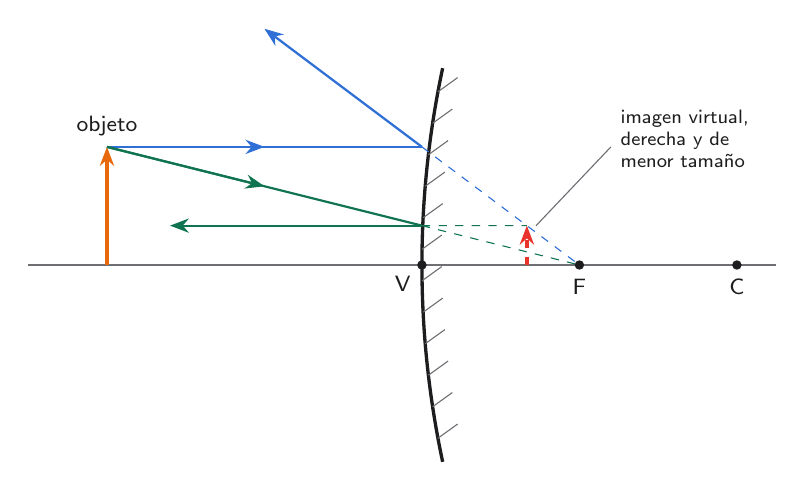
\begin{tikzpicture}[font=\footnotesize,>={Stealth[length=2.4mm]}]
\draw[gris] (-5,0) -- (4.5,0);
\draw[very thick,tinta,domain=-2.5:2.5,samples=60,smooth] plot ({12-sqrt(144-\x*\x)},\x);
\foreach \y in {-2.2,-1.8,...,2.21} \draw[gris,thin] ({12-sqrt(144-\y*\y)},\y) -- ++(0.25,0.18);
\node[below left,text=tinta] at (-0.02,-0.02) {V}; \fill[tinta] (0,0) circle (0.06);
\foreach \x/\t in {2/F,4/C} {\fill[tinta] (\x,0) circle (0.06); \node[below,text=tinta] at (\x,-0.05) {\t};}
\draw[->,line width=1.6pt,nar] (-4,0) -- (-4,1.5) node[above,text=tinta] {objeto};
\draw[azul,thick] (-4,1.5) -- (0,1.5); \draw[->,azul,thick] (-4,1.5) -- (-2,1.5);
\draw[->,azul,thick] (0,1.5) -- (-2,3.0);
\draw[azul,thin,dashed] (0,1.5) -- (2,0);
\draw[menta!70!black,thick] (-4,1.5) -- (0,0.5); \draw[->,menta!70!black,thick] (-4,1.5) -- (-2,1.0);
\draw[->,menta!70!black,thick] (0,0.5) -- (-3.2,0.5);
\draw[menta!70!black,thin,dashed] (0,0.5) -- (2,0) (0,0.5) -- (1.333,0.5);
\draw[->,line width=1.6pt,coral,dashed] (1.333,0) -- (1.333,0.5);
\node[text=tinta,align=left,font=\scriptsize,right] at (2.4,1.6) {imagen virtual,\\derecha y de\\menor tamaño};
\draw[gris,thin] (1.45,0.5) -- (2.4,1.5);
\end{tikzpicture}
\end{document}
